
%\addcontentsline{toc}{chapter}{Anhang}
\cftaddtitleline{toc}{chapter}{Anhang}{}
\pagenumbering{Roman}
\appendix


%\chapter{Ausschreibung Bachelorarbeit}\label{anhang_ausschreibung}
% 
%\includepdf{../ressources/Projektorganisation/Ausschreibung.pdf}
%
%
%\chapter{Projektplanung}  \label{anhang_projektplan} 
%%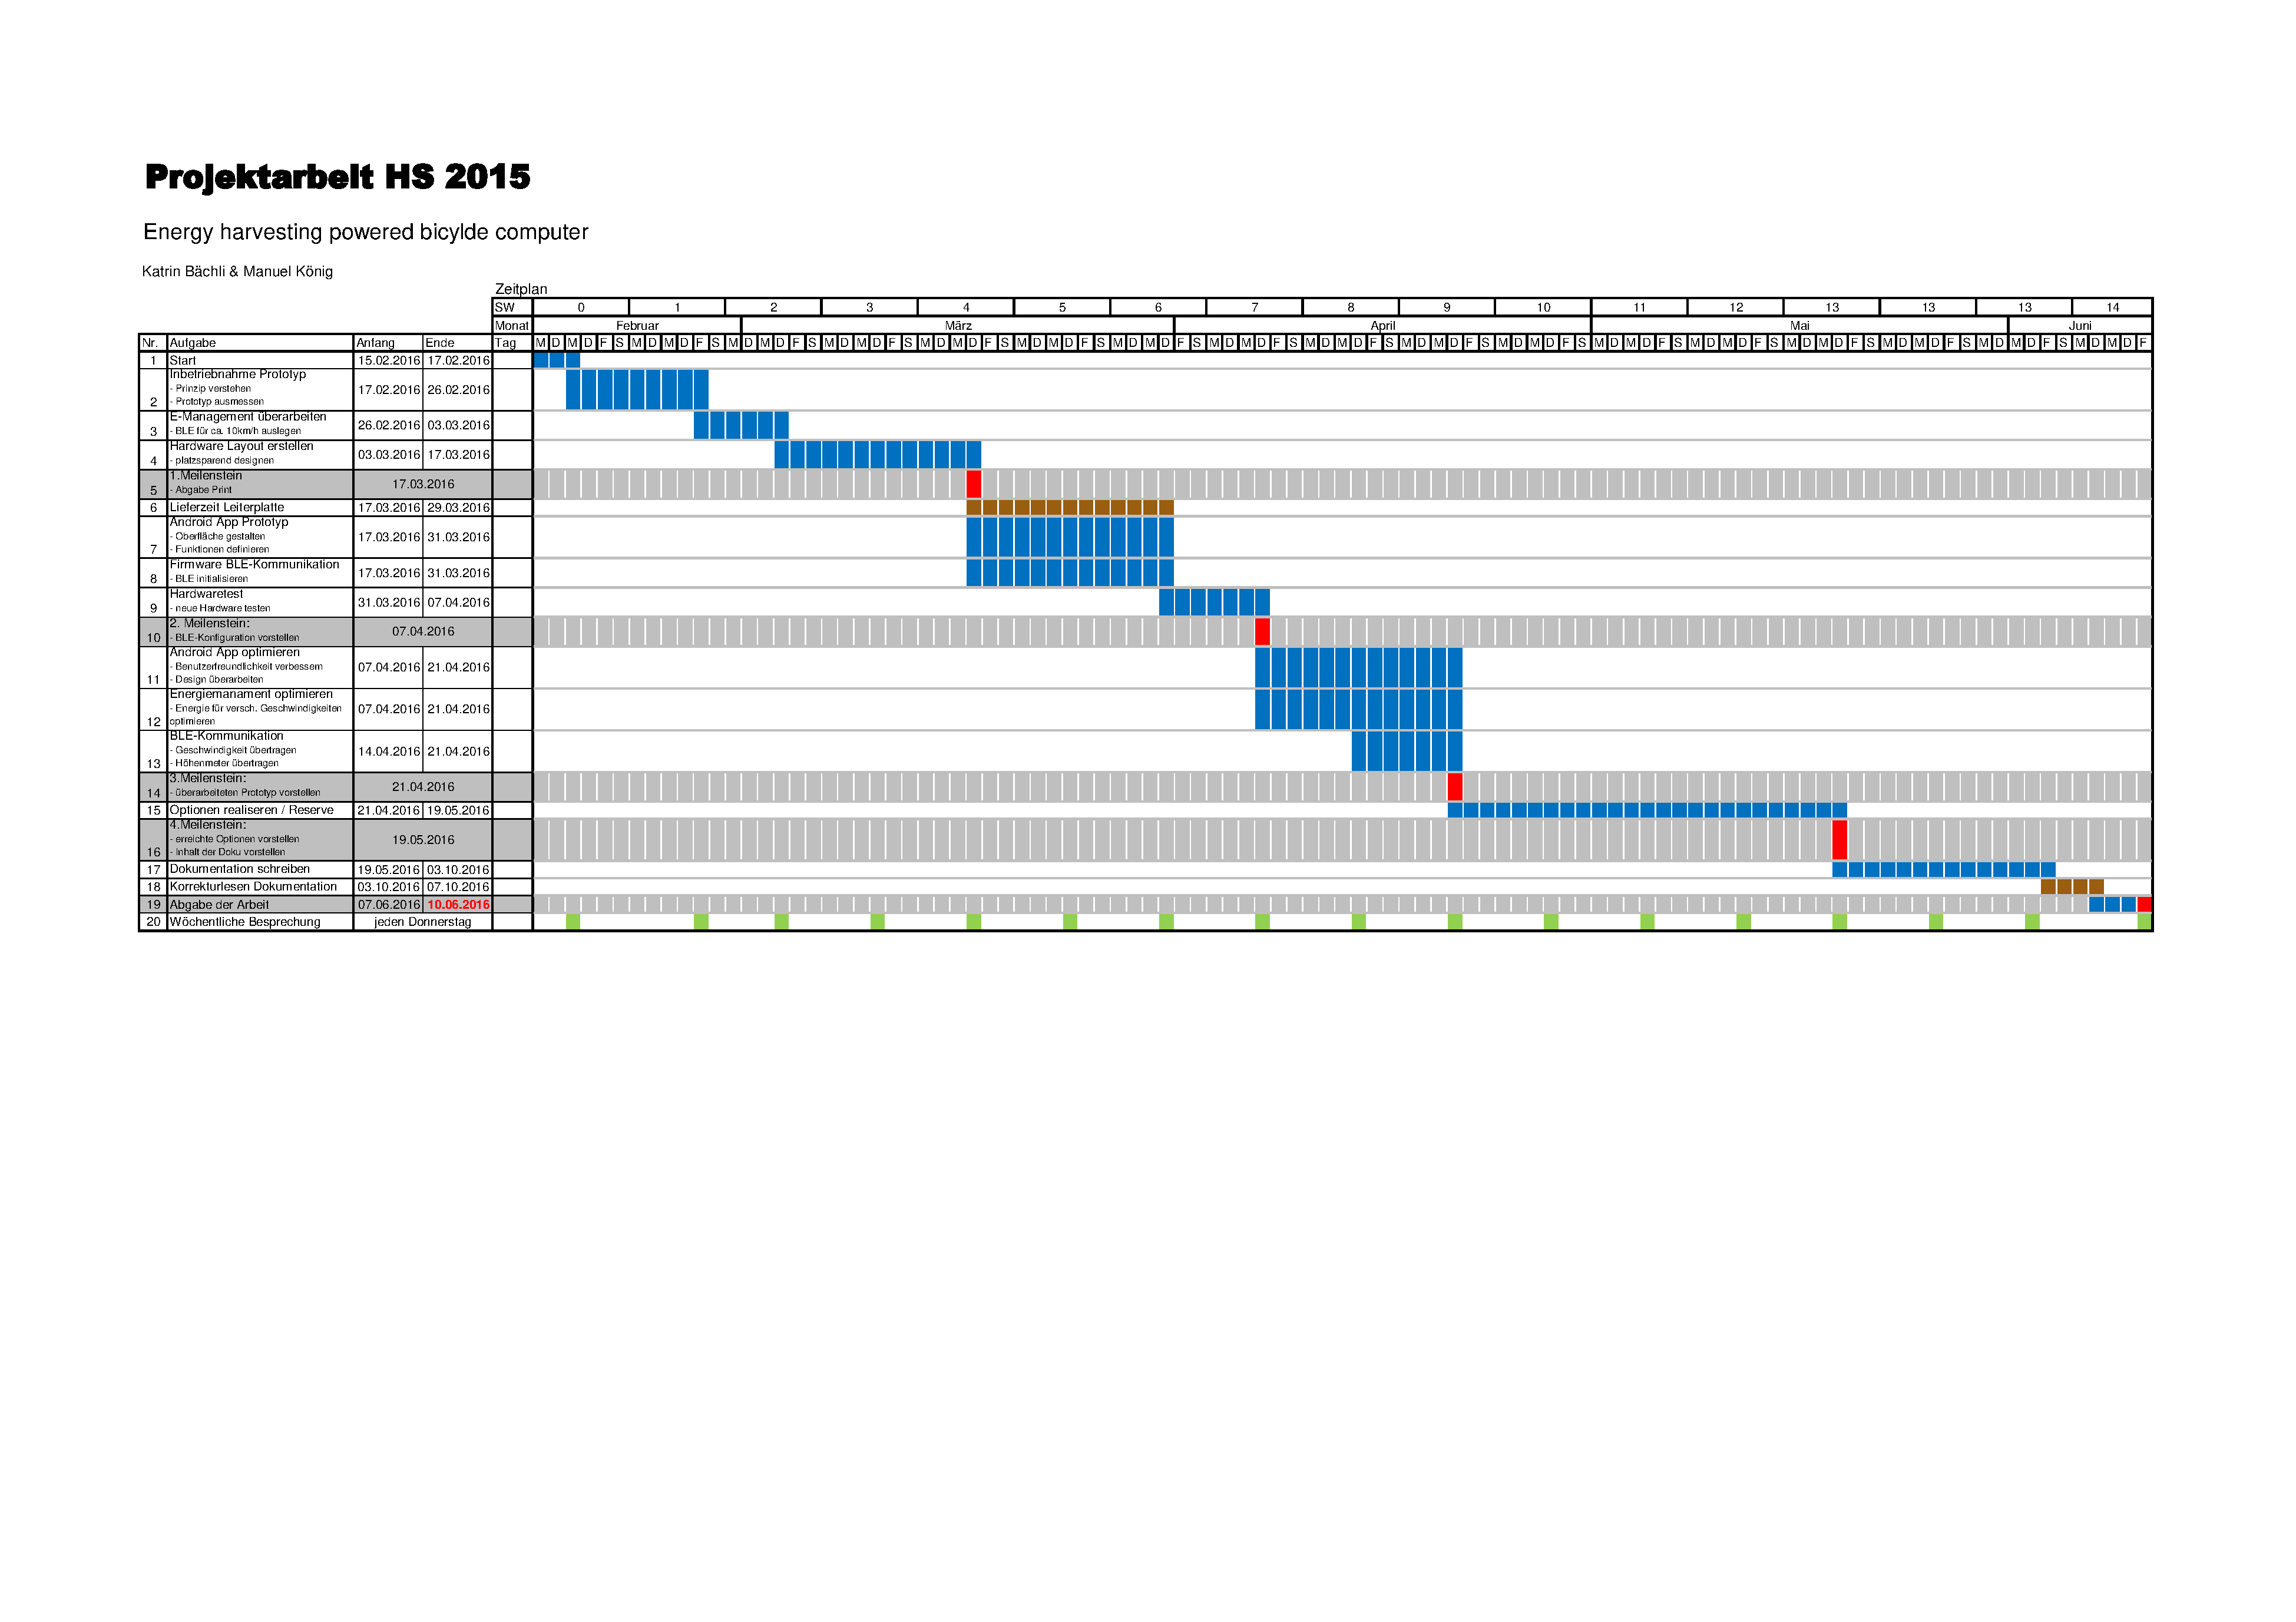
\includepdf [landscape = true, pages=-] {../ressources/Projektorganisation/PlannungV0.pdf}
%
%\vspace*{\fill}\par
%\pagebreak

%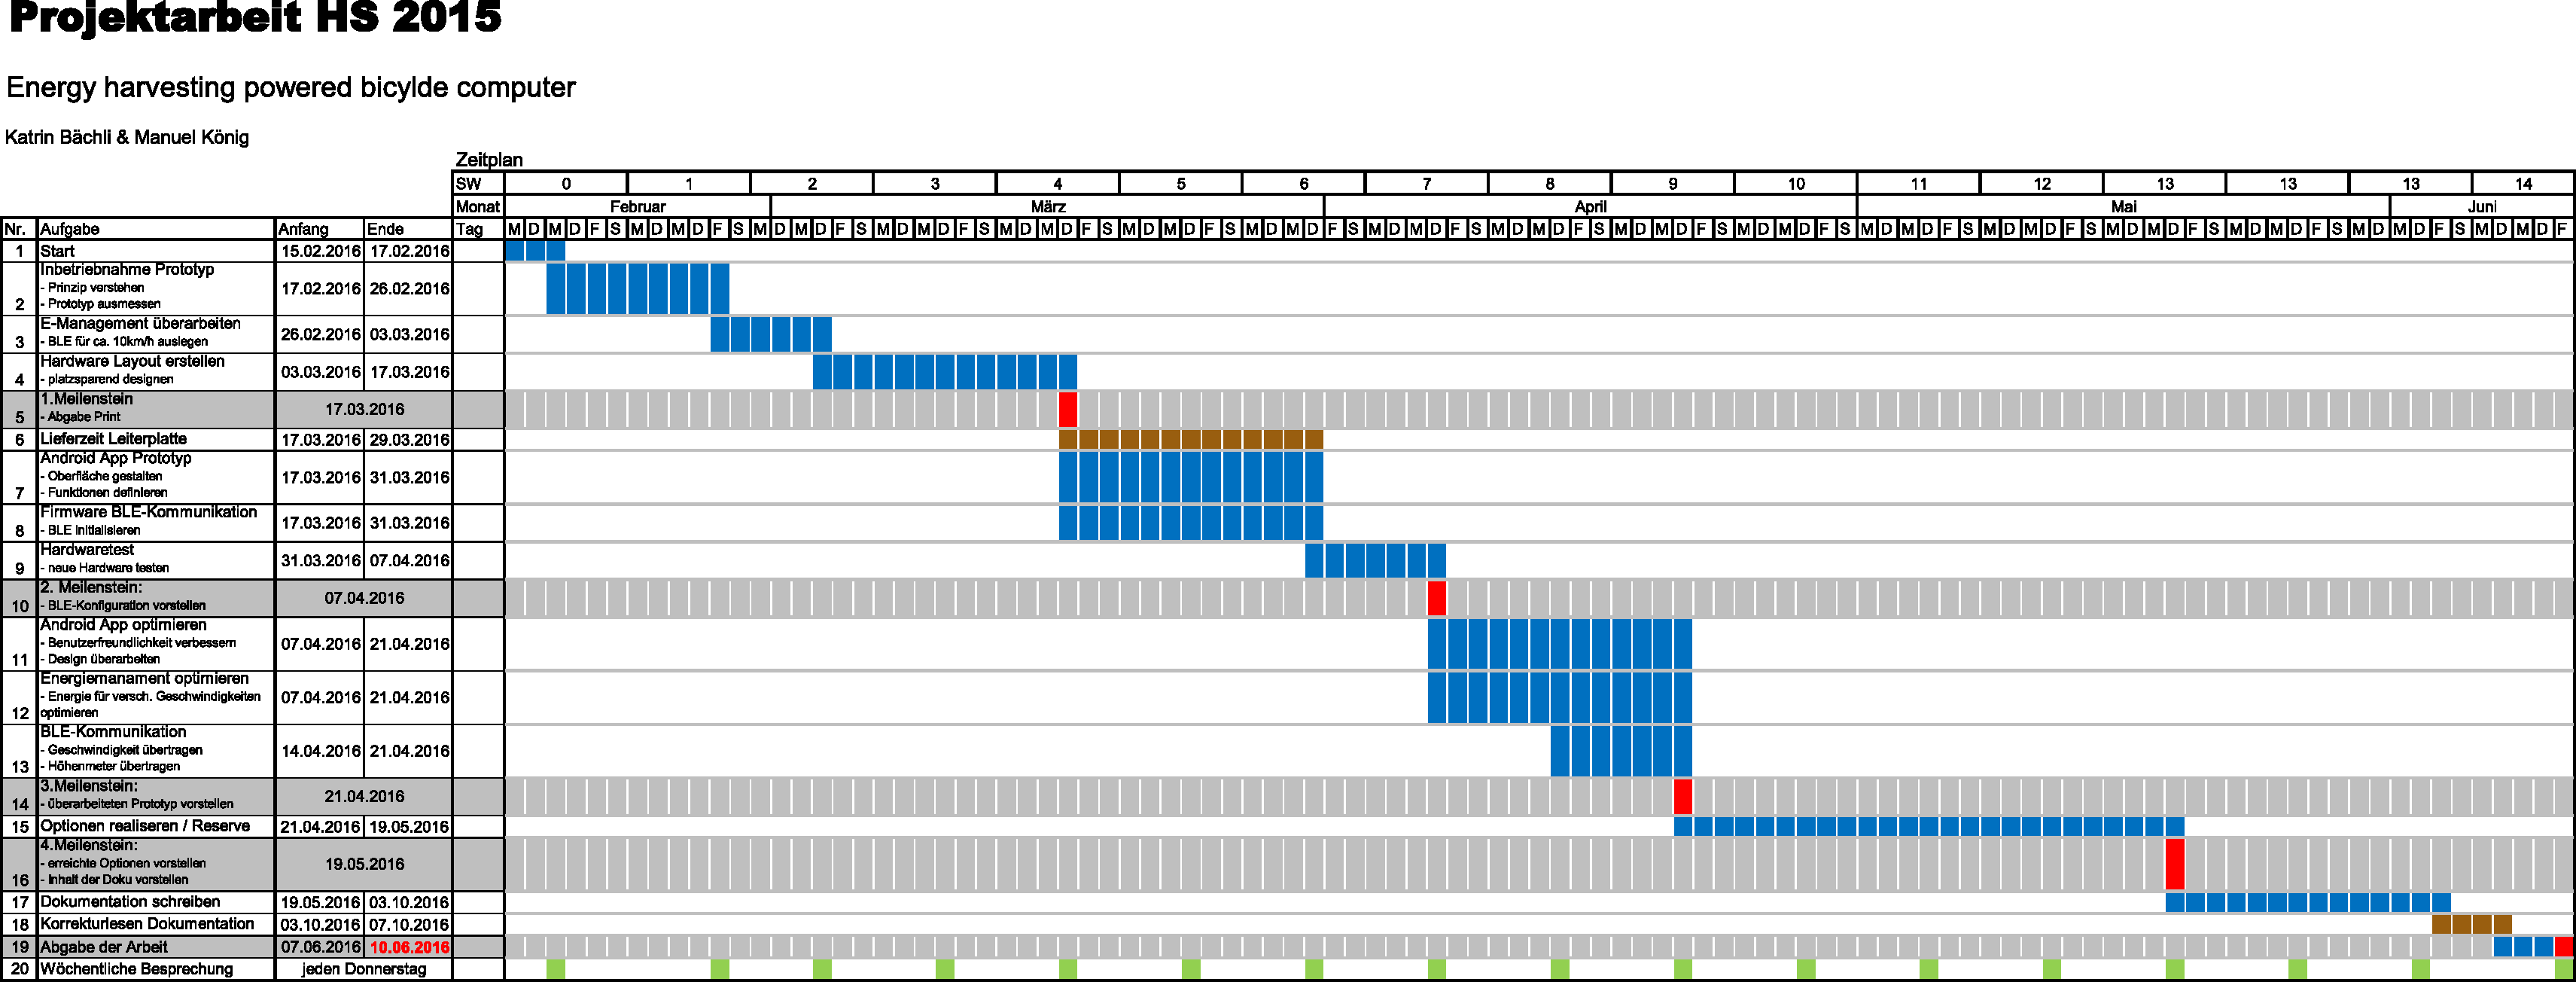
\includegraphics[width=\textheight ,angle=90,origin=c]{../ressources/Projektorganisation/PlannungV0-cropped.pdf}

\chapter{Ausschreibung Bachelorarbeit}

\begin{figure}[h]
    \includegraphics {7Anhang/docs/Ausschreibung.pdf} 
     \caption{Offizielle Ausschreibung der Arbeit}\label{Ausschreibung} 
\end{figure}



\chapter{Blockdiagramm EM8500}\label{anhang_em8500} 
\begin{figure}[h]
    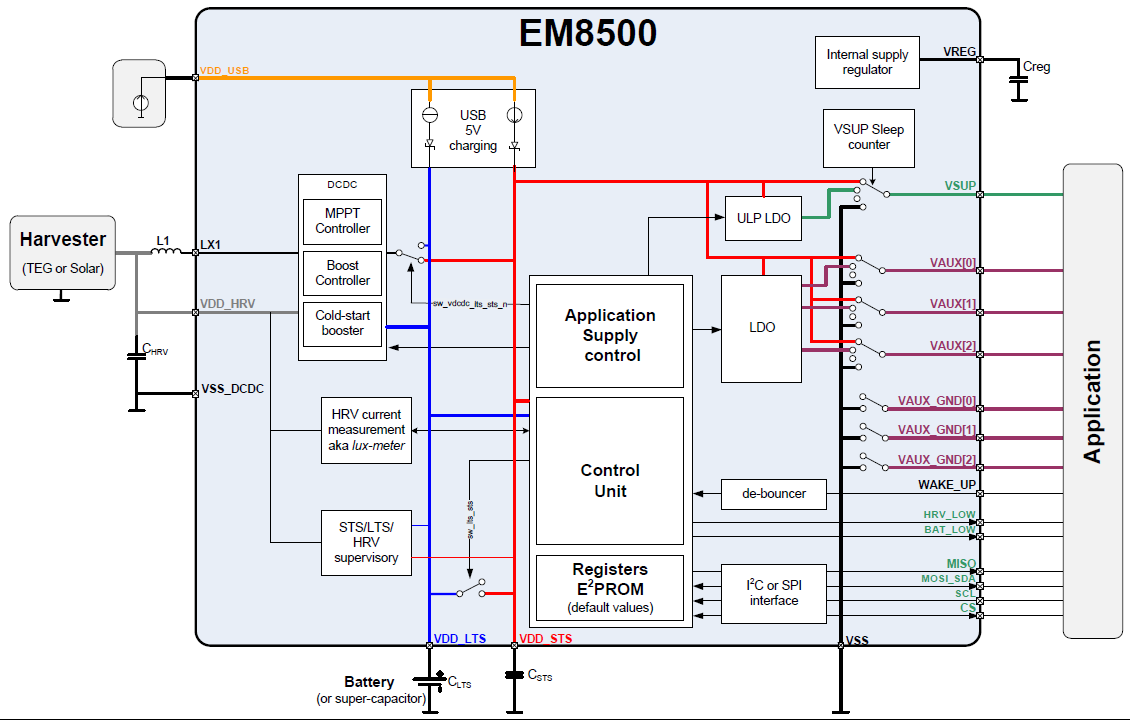
\includegraphics {7Anhang/imag/blockdiagrammEm8500.png} 
     \caption{Blockschema Sensortag}
\end{figure}



\chapter{Funktionsblöcke Sensortag von Texas Instrument}\label{anhang_sensortag} 



\begin{figure}[h]
    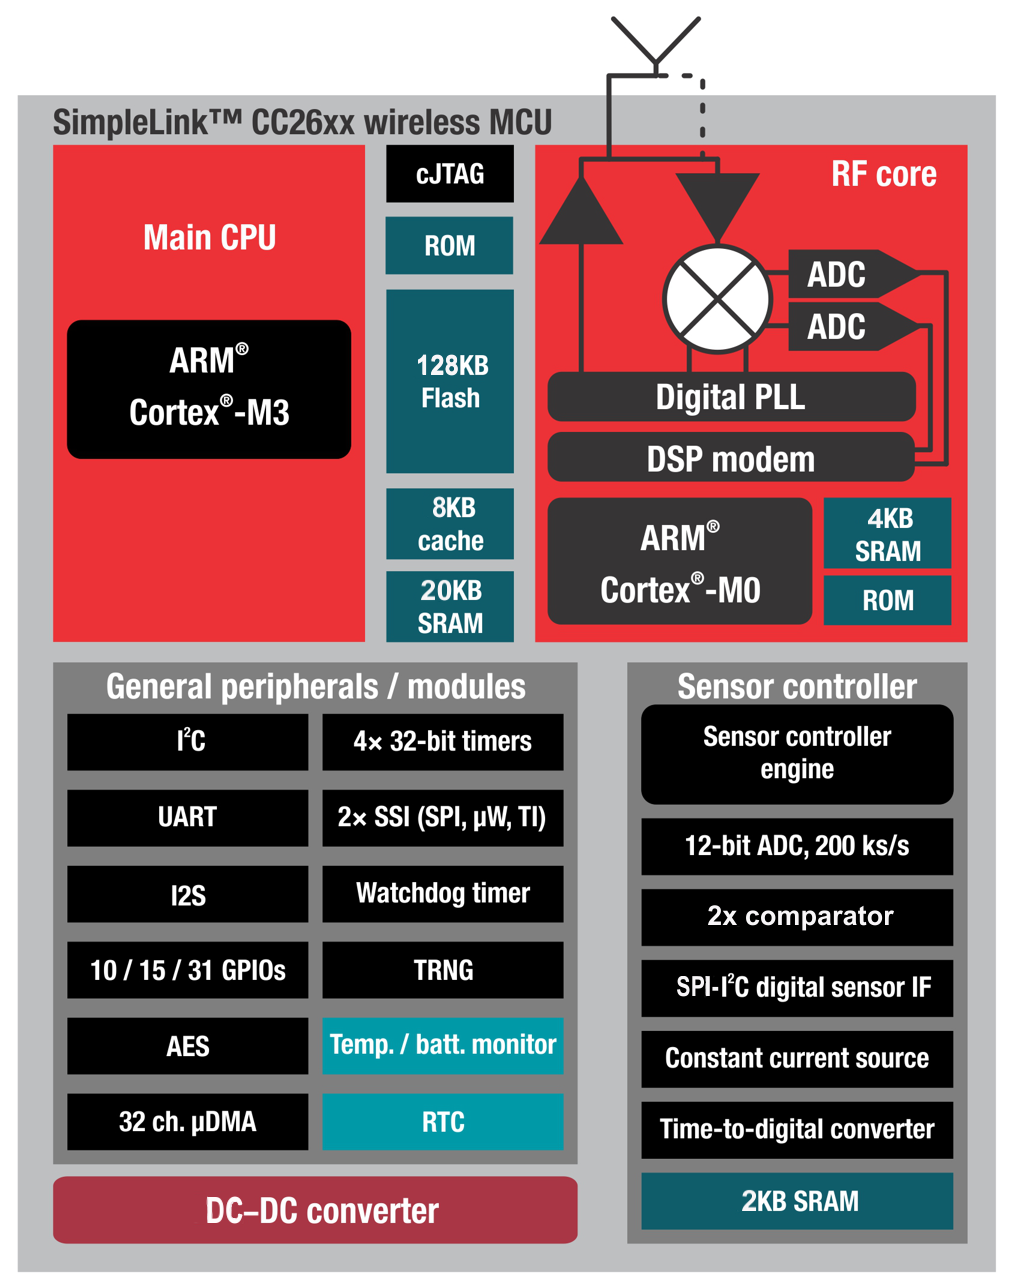
\includegraphics {7Anhang/imag/CC26xx_Block_Diagram.png} 
     \caption{Blockschema Sensortag aus \cite{Sensortag_Datasheet}, S.3}
\end{figure}



\chapter{Messaufbau}
\label{messaufbau}
Problematisch war, dass die Messresultate mit dem Fahrrad nicht reproduzierbar waren, daher wurde eine Radimitation erarbeitet. Herr Erich Ruff hat einen Aubau entwickelt, welcher über einen Elektromotor angetrieben wurde, damit konnte die Geschwindigkeit relativ konstant gehalten werden. Die Toleranz der Geschwindigkeit lag bei +/- 1 km/h, was eine grosse Verbesserung gegenüber der bisherigen Vorgehensweise war.
Die Radimitation bestand aus nur einer Speiche, welche nur eine einfache Alustange war. An dieser Alustange waren mehrere Löcher zur Befestigung des Topfmagneten vorhanden.


\begin{figure}[ht]
    \includegraphics {7Anhang/imag/Messaufbau}
	\caption{Messaufbau während der Inbetriebnahme des Prototypen}
	\label{messaufbau_anhang}
\end{figure}

Der Radimitation ist ein Tachometer angehängt, der die aktuelle Geschwindigkeit anzeigt. Der Tachometer ist vom Hersteller SIGMA Sport, die genaue Bezeichnung Lautet SIGMA SPORT BASELINE 500. Dieser Tachometer wurde im Jahr 1999 hergestellt, funtioniert jedoch nach wie vor einwandfrei.

Im Verlauf der Entwicklung wurde entschieden, dass zwei Magnete im Abstand von 180 Grad angebracht werden. Diese Entscheidung wurde getroffen, um die Energiegewinnung zu maximieren, es wurde jedoch ebenfalls entschieden, dass nicht mehr als zwei Magnete montiert werden sollen. Das Erscheinungbild des Fahrrads würde damit sehr beeinträchtigt und die Bremswirkung würde mit vielen Magneten sicherlich zum Tragen kommen.

Alle Messungen wurden mit einem Radumfang von 2.04 m ausgeführt, der Magnet befand sich 25 cm vom Zentrum der Radsimulation entfernt. Den Einfluss des Abstands kann aus dem Messprotokoll vom 06. Mai 2016 entnommen werden.

\chapter{Übersicht Messprotokolle}
\label{uebersicht_messprotokolle}

\subsubsection*{Übersicht Messprotokolle  }
\label{tabelle_uebersicht_messprotokolle}
\begin{tabbing}
       Messdatum	   	\quad\= Messobjekt    		\quad\= Name des PDF     \\[0.8ex]
       18. Mai 2016 	\> EM8500-Chip-Ausgang 		\> Messprotokoll\_Energiemessung\_EM-Chip\_Inbetriebnahme.pdf\\
	   26. Februar 2016 \> Harvesterausgang Elko 	\> Messprotokoll\_Kondensator\_Ausgang\_Harvesterschaltung.pdf\\
	   14. März 2016 	\> Spule 					\> Messprotokoll\_Optimierung\_Spule.pdf\\
	   14. März 2016 	\> Gleichrichter 			\> Messprotokoll\_Optimierung\_Gleichrichter\_1.pdf\\
	   14. März 2016 	\> Gleichrichter 			\> Messprotokoll\_Optimierung\_Gleichrichter\_2.pdf\\
	   14. März 2016 	\> Spannungsbegrenzung 		\> Messprotokoll\_Optimierung\_Limiter.pdf\\
	   19. März 2016 	\> Harvesterausgang 		\> Messprotokoll\_Leistungskennlinie\_Harvester\_versch\_Harvester.pdf\\
	   30. März 2016 	\> EM8500-Chip-Ausgang 		\> Messprotokoll\_Leistungskennlinie\_Harvester\_kleine\_Spule.pdf\\
	   14. April 2016 	\> Spule und Magnete 		\> Messprotokoll\_Optimierung\_Spule\_versch\_Spulen\_und\_Magnete.pdf\\
	   14. April 2016 	\> Harvesterausgang 		\> Messprotokoll\_Leistungskennlinie\_Harvester\_Prototypenhardware.pdf\\
	   06. Mai 2016 	\> Harvesterausgang 		\> Messprotokoll\_Leistungskennlinie\_Position\_Magnet.pdf\\
	   16. Mai 2016 	\> Prototyp 				\> Messprotokoll\_Inbetriebnahme\_Prototyp.pdf\\
	   16. Mai 2016 	\> Harvesterausgang 		\> Messprotokoll\_Leistungskennlinie\_Harvesterausgang\_Prototyp.pdf\\
	   19. Mai 2016 	\> Prototyp 				\> Messprotokoll\_Inbetriebnahme\_Prototyp\_Energiemanagment.pdf\\
	   21. Mai 2016 	\> Harvesterausgang Elko 	\> Messprotokoll\_Harvesterausgang\_Elko.pdf\\
	   21. Mai 2016 	\> Harvesterausgang 		\> Messprotokoll\_Leistungskennlinie\_Harvesterausgang\_endgültige\_Hardware.pdf\\
	   22. Mai 2016 	\> BLE-Kommunikation 		\> Messprotokoll\_BLE\_Kommunikation\_Paketverlust.pdf\\ %vorhanden
	   28. Mai 2016 	\> EM8500-Chip-Ausgang 		\> Messprotokoll\_Energiemessung\_EM-Ausgang\_endgültige\_Hardware.pdf\\ %vorhanden
	   03. Juni 2016 	\> TI-SensorTag 			\> Messprotokoll\_Energieverbrauch\_Sensortag.pdf\\
\end{tabbing}  